\section{Architecture overview}
In order to make packages in Columbus lay user friendly and programming language independent, they 
are designed as web applications with a graphical user interface. These apps can optionally expose REST 
endpoints as microservices. These microservices can be chained together to create custom workflows.

In this section, we present an overview of the achritecture of Columbus and its ecosystem of apps,
which was designed to meet the criteria identified in the previous section.

\begin{figure}[t]
  \caption{Columbus architecture overview}
  \centering
  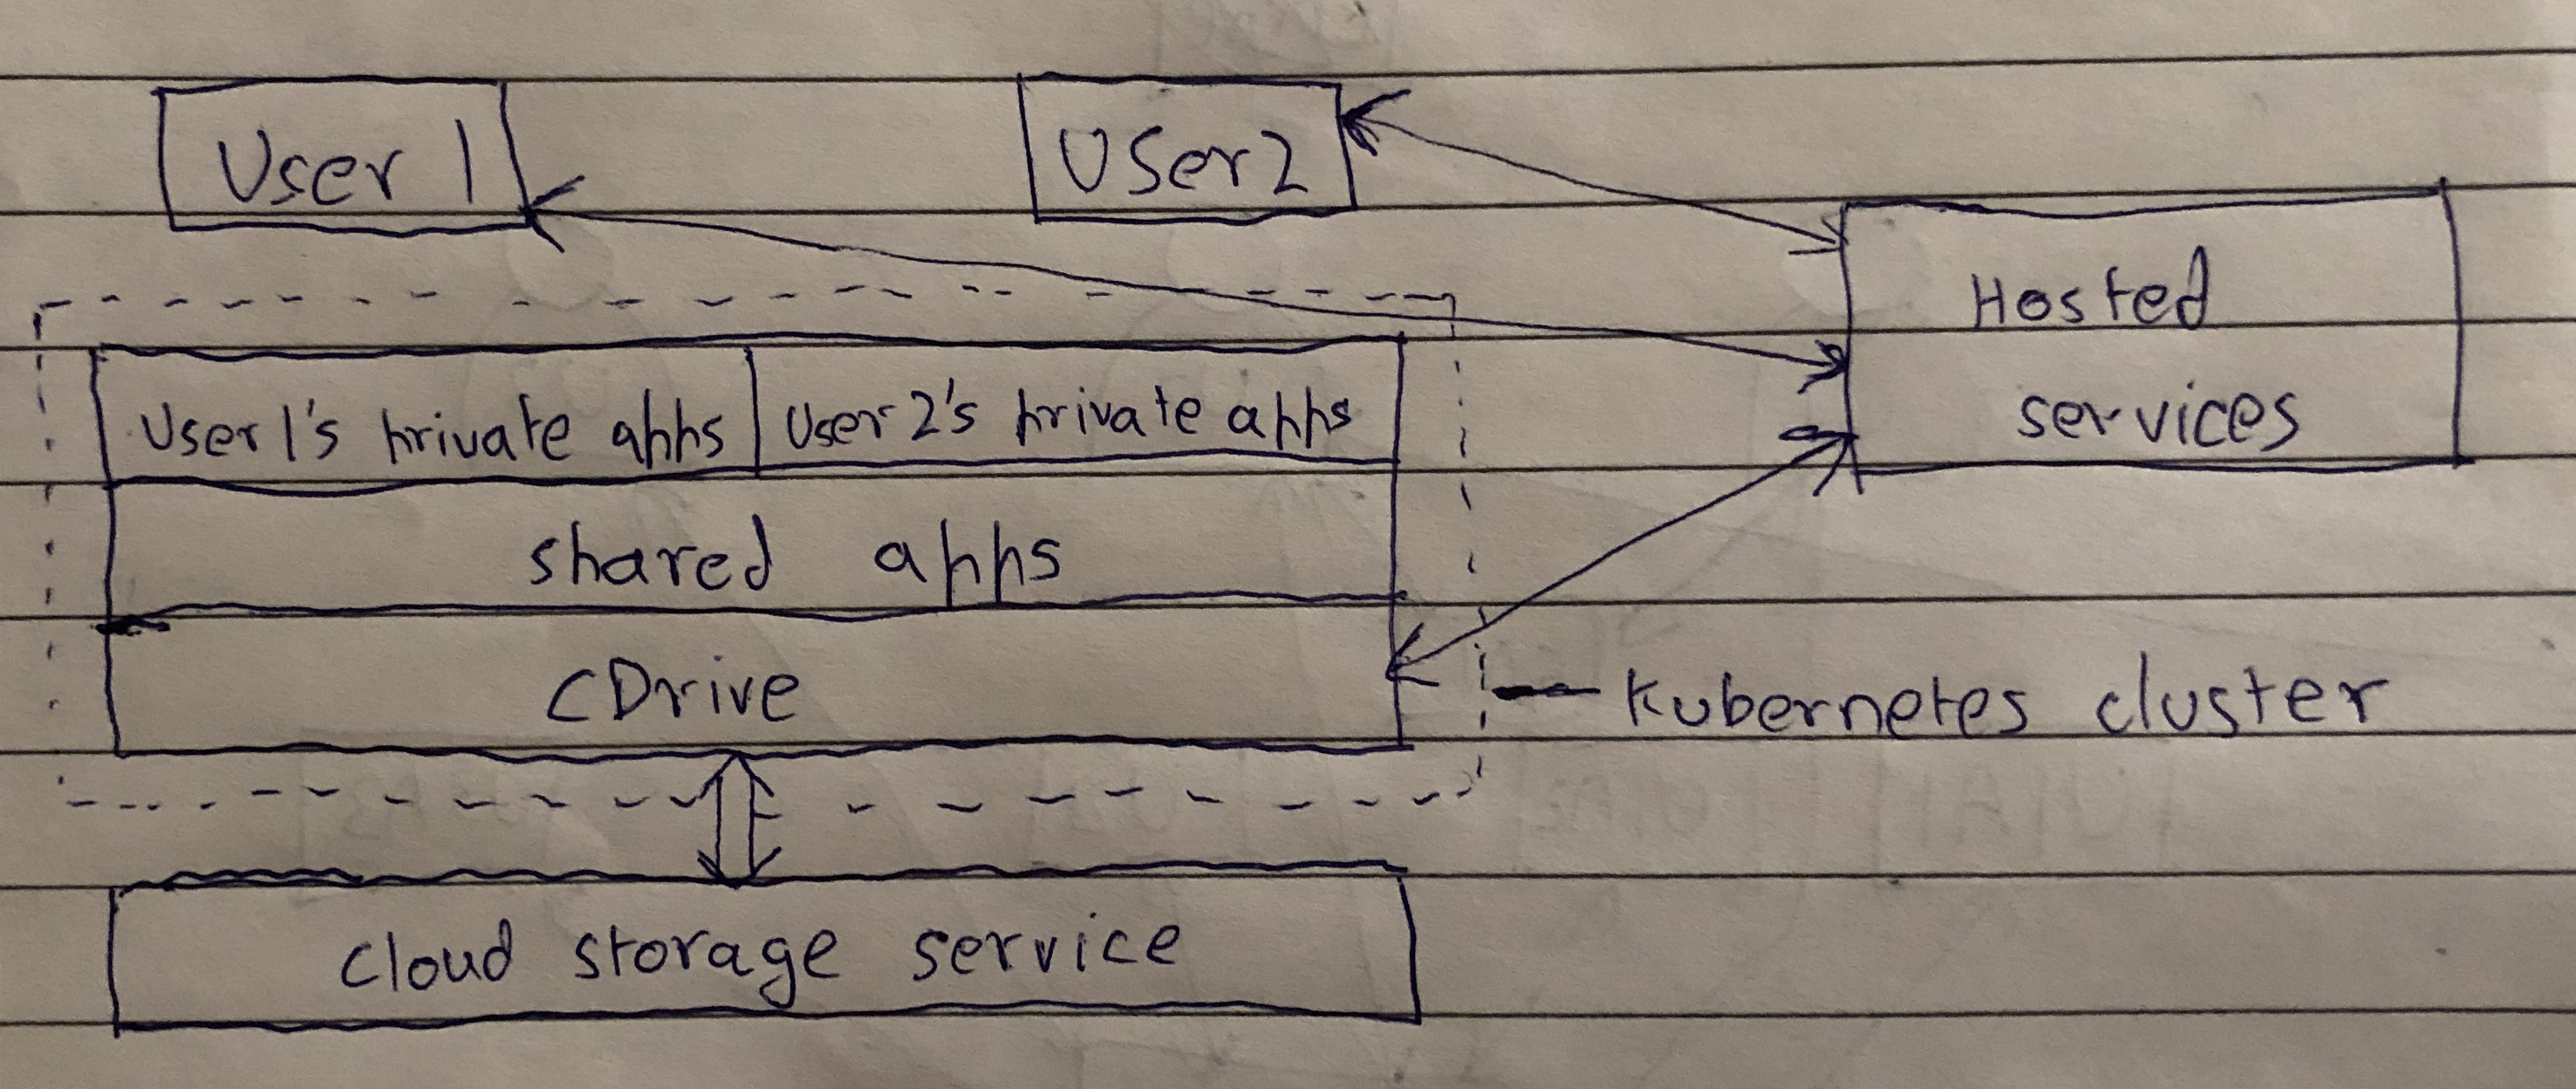
\includegraphics[width=7cm, height=4cm]{arch-overview}
\end{figure}

\subsection{Columbus on Kubernetes}

Columbus is designed to run on a Kubernetes cluster due to the following reasons:
\begin{itemize}
  \item We want system administrators to be able to easily scale a Columbus deployment up or down 
    without needing additional efforts from an infrastructure team. Running on an established 
    container orchestration platform allows a Columbus deployment to serve a small team of 5 or a
    large team of hundreds of users without any change in the deployment process. It also allows
    an already existing deployment to dynamically scale up or down as per requirements.
  \item We wanted individual components of Columbus to function as independently as possible. In 
    keeping with the current best programming practices, we built the Colummbus platform itself as a 
    collection of microservices. A Kubernetes cluster provides an internal network for easy and 
    secure communication between these microservices running on the cluster.
  \item In order to allow individual apps to run within a consistent environment, they are run as
    containers within a Kubernetes cluster. Kubernetes provides a lot of ready made machinery for 
    managing the lifecycle of these apps.
  \item We wanted Columbus apps to be easy to install, so we require that they are packaged as
    container images which individual users can pull and install for their personal use on Columbus.
    Kubernetes provides authentication and security machinery that allows us to implement this in
    a secure way.
  \item We want apps to be able to expose microservices, which can then be composed together to 
    create new apps that can execute more detailed workflows. Exposing these microservices over a
    Kubernetes cluster makes it easy to dynamically scale them depending on usage. Kubernetes also
    allows replicating these microservice and load balancing between replicas in order to make them
    highly available with no down time.
  \item Kubernetes allows multiplexing of cluster resources between different applications as well
    as the Columbus platform without a particularly extensive setup procedure and Kubernetes also
    takes care of load balancing over the cluster.
  \item Kubernetes allows system adminsitrators to perform rolling updates to an existing Columbus
    deployment, for example to upgrade to a newer version of Columbus with zero down time.
  \item A Kubernetes cluster can be set up on a local machine, over an on-premise network or over
    public cloud infrastructure. Designing Columbus to run on Kubernetes allows gives users the 
    flexibility to choose their preferred infrastructure over which to deploy Columbus.
  \item Kubernetes provides fairly comprehensive logging facilities out of the box, which we
    leverage to make continuous improvements to the system.
\end{itemize}

\subsection{Columbus drive overview}
Once a Kubernetes cluster has been set up and Columbus has been deployed on it, users can come in
and create accounts on the platform. Each Columbus account has a Columbus Drive (abbreviated as 
CDrive) associated with it. Users can upload files and folders to their CDrive. Users can also 
share data with other users. Edit or view permissions can be provided on the data or a user may
also choose to make some data available publically outside the Columbus deployment.


Columbus consists of CDrive and applications which carry out some kind of processing on the data 
within CDrive. Users can install applications on their CDrive account. By default, applications 
cannot access a user's data. Users can choose which folders within their CDrive can be accessed 
by each application. 

\subsection{Columbus applications overview}

CDrive allows three kinds of applications, namely, private applications, hosted applications and
shared applications.

\subsubsection{Private applications}
Private apps are apps that are private to each user. App developers create the apps as docker 
images and publish them to an online container image repository such as DockerHub or Google 
Container Registry. A Columbus user can install these apps from within their CDrive. When a 
user installs a private app, CDrive pulls the app image from the image repository and deploys
it on the same Kubernetes cluster on which CDrive is running. CDrive also sets up a URL on which
the newly installed app can be accessed and creates an entry on the user's CDrive account which
links to the application URL. These apps are per-user instances i.e. if two users install the 
same container image, two separate instances of the container are run on the Kubernetes cluster,
and each instance doesn't know about the other.

\subsubsection{Shared applications}
Shared applications are applications that are common to all user accounts on a particular Columbus
deployment. These applications cannot be installed from within a user account, they need to be
set up by the system administrator. Once a shared application has been set up, any user can come
in and use this application from their Columbus account. 


Shared applications would typically
require more cluster resources than private applications and/or more specific, highly customized 
deployment as well. Only one instance of a shared application exists for all users within a single
Columbus deployment, so a shared application is expected to carry out its own authentication and
authorization although it can use the third party authentication service provided by Columbus. A 
shared application is also expected to carry out its own load balancing and replication, although
this is easy to do on a Kubernetes cluster. 


Shared applications provide a way to customize the functionality of the platform at the
infrastructure level. An organization could fork the publicly available source code for Columbus,
add some custom shared applications tailored to the requirements of their users and deploy it on
a Kubernetes cluster, thus creating a customized Columbus deployment.

\subsubsection{Hosted applications}
Private and shared applications are run on the same cluster as CDrive. But, we also wanted to 
allow users to optionally use some commercial/close sourced services to operate on their CDrive
data. These are termed as hosted applications as they will be hosted on infrastructure external to
the Columbus platform. Hosted applications will need to expose a URL and follow certain rules in
order to be CDrive compliant. Users will then be able to create an account on the hosted application
and link that account with their Columbus account. The hosted app vendor may optionally impose 
restrictions on its usage such as a fee per unit usage, or a free trial version with a charge for
the premium version. Similar to private apps, hosted apps may also optionally expose some REST 
endpoints as microservices which can be chained together in workflows and scripts.

\subsection{Jupyter Notebook}
CDrive also contains a Jupyter Notebook interface. Users can use this interface to 
programmatically make calls to microservices exposed by CDrive and its ecosytem of applications.
This interface can be used for chaining together multiple apps to create workflows, executing the
workflows as well as saving the workflow to CDrive and sharing it with other users.
